%%%%%%%%%%%%%%%%%%%%%%%%%%%%%%%%%%%%%%%%%
% Template information:
% Template name: Ernie's Beamer
% Version: 1.0 (2023.03.24)
% Editor: 莊程翔 Ernie Cheng-Xiang Zhuang
% Complier: XeLaTeX
%
% Original Template Information:
% Template name: Beamer Presentation
% Author: Vel (vel@latextemplates.com)
% Complier: XeLaTeX
% License: CC BY-NC-SA 4.0 (https://creativecommons.org/licenses/by-nc-sa/4.0/)
% Download link: https://www.LaTeXTemplates.com
%
% The purpose of making this template:
% Due to the unfriendliness of LaTeX for beginners, I made significant modifications to the template designed by Vel, along with clear and concise comments. I also added many commonly used and useful packages, as well as frequently used customized settings commands, to make it easier for LaTeX beginners to complete professional academic presentations.
% If you have any questions, you can contact me by:
% 1. Website: https://www.ernie-zhuang.com/contact
% 2. Email: erniezhuang1127@gmail.com
%%%%%%%%%%%%%%%%%%%%%%%%%%%%%%%%%%%%%%%%%

%----------------------------------------------------------------------------------------
%	Packages and Document Configurations
%----------------------------------------------------------------------------------------

% font size 12pt (It can be changed to: 8pt、9pt、10pt、11pt (default)、12pt、14pt、17pt or 20pt)
% Set the ratio to be 16:9 (It can be changed to: 1610、149、54、43 (default) or 32)
% If animation is set up and needs to be output, remember to add 'handout' to avoid printing too many similar pages.
\documentclass[12pt, aspectratio=169]{beamer} 

%%%%%%%%%%%%%%%%%%%%%%%%%%%%%%%%%%%%%%%%%
% Template information:
% Template name: Ernie's Beamer
% Version: 1.0 (2023.03.23)
% Editor: 莊程翔 Ernie Cheng-Xiang Zhuang
% Complier: XeLaTeX
%
% Original Template Information:
% Template name: Beamer Presentation
% Author: Vel (vel@latextemplates.com)
% Complier: XeLaTeX
% License: CC BY-NC-SA 4.0 (https://creativecommons.org/licenses/by-nc-sa/4.0/)
% Download link: https://www.LaTeXTemplates.com
%
% The purpose of making this template:
% Due to the unfriendliness of LaTeX for beginners, I made significant modifications to the template designed by Vel, along with clear and concise comments. I also added many commonly used and useful packages, as well as frequently used customized settings commands, to make it easier for LaTeX beginners to complete professional academic presentations.
% If you have any questions, you can contact me by:
% 1. Website: https://www.ernie-zhuang.com/contact
% 2. Email: erniezhuang1127@gmail.com
%%%%%%%%%%%%%%%%%%%%%%%%%%%%%%%%%%%%%%%%%

%----------------------------------------------------------------------------------------
%	Packages and Document Configurations
%----------------------------------------------------------------------------------------

% Specification of custom fonts
\usepackage{fontspec} 

%% Specified font
\usefonttheme{serif} % Typeset using the default serif font

% Required for custom colors
\usepackage{color} 

%% Color section titles
\definecolor{NTHU_Purple}{RGB}{126,35,138}
\definecolor{Default_Blue}{RGB}{52,51,171}

% Math tools and symbols
\usepackage{mathtools, amsmath, amsfonts, amsthm, latexsym} 

% Increase the space between mathematical symbols and make the ones bold
\usepackage{newtxtext, newtxmath}

% Automatic numbering of figures and tables
\usepackage[justification=centering]{caption} 
\usepackage[justification=centering, format=hang]{subcaption}

%% Set the automatic numbering
\setbeamertemplate{caption}[numbered]

%% Set the font size and series of automatic numbering
\captionsetup[figure]{font=small, labelfont=md}
\captionsetup[table]{font=small, labelfont=md}

% Packages of tables and figures
\usepackage{graphicx}  % \scalebox{} can resize a table
\usepackage{booktabs}

%Arrange multiple figures
\usepackage{subfigure} 

% Multiple row
\usepackage{multirow} 

% Array
\usepackage{array}

% Enumerate
\usepackage{enumerate} 

% For making a watermark
\usepackage{tikz}

% References
\usepackage{natbib}

% Commenting out large sections
\usepackage{comment}

%----------------------------------------------------------------------------------------
%	Layout theme (Select one)
%----------------------------------------------------------------------------------------

\mode<presentation>{
%\usetheme{default}
%\usetheme{AnnArbor}
%\usetheme{Antibes}
%\usetheme{Bergen}
%\usetheme{Berkeley}
%\usetheme{Berlin}
%\usetheme{Boadilla}
%\usetheme{CambridgeUS}
%\usetheme{Copenhagen}
%\usetheme{Darmstadt}
%\usetheme{Dresden}
%\usetheme{Frankfurt}
%\usetheme{Goettingen}
%\usetheme{Hannover}
%\usetheme{Ilmenau}
%\usetheme{JuanLesPins}
%\usetheme{Luebeck}
\usetheme{Madrid}
%\usetheme{Malmoe}
%\usetheme{Marburg}
%\usetheme{Montpellier}
%\usetheme{PaloAlto}
%\usetheme{Pittsburgh}
%\usetheme{Rochester}
%\usetheme{Singapore}
%\usetheme{Szeged}
%\usetheme{Warsaw}

%----------------------------------------------------------------------------------------
%	Outer theme (Select one)
%----------------------------------------------------------------------------------------

%\useoutertheme{default}
%\useoutertheme{infolines}
%\useoutertheme{miniframes}
\useoutertheme{smoothbars}
%\useoutertheme{sidebar}
%\useoutertheme{split}
%\useoutertheme{shadow}
%\useoutertheme{tree}
%\useoutertheme{smoothtree}

%----------------------------------------------------------------------------------------
%	Custom outer theme
%----------------------------------------------------------------------------------------

% Set the font color black and background black in headline and footline
%\setbeamercolor{section in head/foot}{fg=black, bg=white} 

% Cancel the counter of page in sections
%\setbeamertemplate{mini frames}{}  

% Adjust the font size of headline and footline
\setbeamerfont{headline}{size=\scriptsize}
\setbeamerfont{footline}{size=\scriptsize}

% Cancel the page toolbox out
\setbeamertemplate{navigation symbols}{} 

%% Customization 1: The footline just contains author and page  
%\setbeamertemplate{footline} 
%{\leavevmode%
%\hbox{%
%\begin{beamercolorbox}[wd=0.5\paperwidth,ht=3ex,dp=1ex,leftskip=3ex]%
%{author in head/foot}%
%{\scriptsize\textbf{\insertshortauthor}}%
%\end{beamercolorbox}%
%\begin{beamercolorbox}[wd=0.5\paperwidth,ht=3ex,dp=1ex,right]%
%{author in head/foot}%
%\scriptsize \textbf{{\insertframenumber{} / \inserttotalframenumber\hspace*{2ex}}} %頁碼控制選項
%\end{beamercolorbox}%
%}}

%% Customization 2: Clear the footline but leave the page
%\setbeamertemplate{footline}[page number] 

%% Customization 3: Clear the ffootline
%\setbeamertemplate{footline}[] 

%----------------------------------------------------------------------------------------
%	Color theme (Select one)
%----------------------------------------------------------------------------------------

\usecolortheme{default}
%\usecolortheme{albatross}
%\usecolortheme{beaver}
%\usecolortheme{beetle}
%\usecolortheme{crane}
%\usecolortheme{dolphin}
%\usecolortheme{dove}
%\usecolortheme{fly}
%\usecolortheme{lily}
%\usecolortheme{orchid}
%\usecolortheme{rose}
%\usecolortheme{seagull}
%\usecolortheme{seahorse}
%\usecolortheme{whale}
%\usecolortheme{wolverine}

%----------------------------------------------------------------------------------------
%	Custom color theme
%----------------------------------------------------------------------------------------

% The structure color (You can change the color to fit the represent color of institute or school)
\setbeamercolor{structure}{fg=NTHU_Purple} 

% Change the color of font and title block in title page
%\setbeamercolor{title}{bg=green, fg=black} 

% Change the color of font and frametitle block
%\setbeamercolor{frametitle}{bg=green,fg=black} 

% Change the context color
%\setbeamercolor{normal text}{fg=orange}

% Change the color of font and the background in the title of block 
%\setbeamercolor{block title}{bg=blue,fg=yellow} 

% Change the color of font and the background in the body of block 
%\setbeamercolor{block body}{bg=green,fg=red} 

% Set the color for alerted text
\setbeamercolor{alerted text}{fg=red} 

%----------------------------------------------------------------------------------------
%	Inner theme (Select one)
%----------------------------------------------------------------------------------------

\useinnertheme{rounded} 
%\useinnertheme{circles} 
%\useinnertheme{rectangles} 
%\useinnertheme{inmargin} 

%----------------------------------------------------------------------------------------
%	Custom item color
%----------------------------------------------------------------------------------------

%\setbeamercolor{item projected}{bg=red}

%----------------------------------------------------------------------------------------
%	Custom the margin of slides
%----------------------------------------------------------------------------------------

\setbeamersize{text margin left=0.8cm, text margin right=0.8cm}
\special{papersize=\the\paperwidth,\the\paperheight}
\providecommand{\tabularnewline}{\\}
}

%----------------------------------------------------------------------------------------
%	Custom the background
%----------------------------------------------------------------------------------------

% Add background picture
%\setbeamertemplate{background}{
\includegraphics[height=\paperheight]{Fig/Background.png}}

% Set the watermark
\usebackgroundtemplate{%
	\tikz[overlay, remember picture] % Show the logo at every page
	\node[opacity=0.3, below=-1.25cm, at=(current page.center)] % Adjust the opacity and position
	{
\includegraphics[scale = 0.14]{Fig/nthulogo.png}}; % input the logo and change size
	}
 % Input packages and our setting in structure.tex

\begin{document}

%----------------------------------------------------------------------------------------
%	Presentation Information
%----------------------------------------------------------------------------------------

% [] : The content will be showed in headline or footline
% {} : The content will be showed in title slide

% Title
\title[How to do the \LaTeX{}  Beamer?]{\Huge{\textbf{How to do the \LaTeX{}  Beamer?}}} 

% Subtitle
\subtitle{Various page templates that may be required} 

% Author(s)
\author[Ernie Cheng-Xiang Zhuang]{% 
Ernie Cheng-Xiang Zhuang one \thanks{National Tsing Hua University one} \and%
Ernie Cheng-Xiang Zhuang two \thanks{National Tsing Hua University two}
}

% Institute
\institute[NTHU]{\normalsize National Tsing Hua University} 

% Date
\date[\today]{\today}

%----------------------------------------------------------------------------------------
%	Title Slide
%----------------------------------------------------------------------------------------

\begin{frame}
	\titlepage % Print the title slide
\end{frame}

%----------------------------------------------------------------------------------------
%	Table of Contents
%----------------------------------------------------------------------------------------

\begin{frame}{\textbf{Table of Contents}}
	\tableofcontents % Print the all sections and subsections
\end{frame}

%----------------------------------------------------------------------------------------
%	(Animation) Words will be displayed faintly
%----------------------------------------------------------------------------------------

\beamersetuncovermixins{\opaqueness<1->{45}}{\opaqueness<1->{95}} 

%----------------------------------------------------------------------------------------
%	Sentence
%----------------------------------------------------------------------------------------

\section{Sentence}

%----------------------------------------------------------------------------------------

\linespread{1}  % After this line, it will be 1 times the line height
\begin{frame}{\textbf{Sentence}}
\linespread{1.5} % After this line, it will be 1.5 times the line height
	
	% \alert can make the words appear in red
	% \textbf can make the words appear in bold
	% \textit can make the words appear in italics
	 \alert{Econometrics} is a \textbf{statistical} method used to \textit{estimate} the economic relationship,
	 test economic theories, and evaluate the effects of government or business policies.
	 
	 % (Animation) This command displays the sentences that have been entered so far.
	 \pause 
	
	% Vertical whitespace (It can be changed to: \medskip, \smallskip, \vspace{?em}))
	\bigskip 
	
	% quote
	\begin{quote}
		Pure mathematics is, in its way, the poetry of logical ideas.\\
		--- Albert Einstein
	\end{quote}
	
\end{frame}

%----------------------------------------------------------------------------------------
%	Itemize and Enumerate
%----------------------------------------------------------------------------------------

\section{Itemize and Enumerate}

%----------------------------------------------------------------------------------------

% [<+>] will automatically animate, so you don't have to keep typing \pause.
\linespread{1} 
\begin{frame}[<+>]{\textbf{Itemize and Enumerate}}
\linespread{1.5} 

	\begin{itemize}[] % item of `itemize' package
		\item This is an item of `itemize' package
		\begin{enumerate}[] % item of `enumerate' package with typing null in []
			\item This is an item in the `enumerate' package
			\item You can compare both:
				\begin{enumerate}[1] % item of 'enumerate' package with typing 1 in []
					\item The items in the `itemize' package appear smaller in size
					\item The items in the `enumerate' package appear bigger in size
					\item In addition, you may observe that words appear smaller when they are positioned closer to the center.
				\end{enumerate}
		\end{enumerate}
	\end{itemize}
	
\end{frame}

%----------------------------------------------------------------------------------------
%	Math Block
%----------------------------------------------------------------------------------------

\section{Math}

%----------------------------------------------------------------------------------------

\linespread{1}
\begin{frame}{\textbf{Math Block}}
\linespread{1.5} 

	\begin{block}{\textbf{Definition}} 
		Let $f\left(x\right)$ be a function defined on an interval that contains $x=c$,
		except that possibly at $x=c$. Then we say that,
		$\lim\limits_{x\rightarrow c} f\,(x)=L$
		if for every number $\epsilon > 0$ there is some number  $\delta > 0$ such that
		$\left\vert f(x)-L \right\vert < \epsilon$ whenever $0<\left\vert x-c \right\vert < \delta$
	\end{block}
	
	\begin{definition}
		You can also use \textbackslash{}begin\{definition\} and \textbackslash{}end\{definition\} to write definitions,
		but it may be difficult to change the title formatting,
		such as making it appear in bold.
	\end{definition}
	
\end{frame}

%----------------------------------------------------------------------------------------

\linespread{1}
\begin{frame}{\textbf{Math Block (Con't)}}
\linespread{1.5} 

	\begin{block}{\textbf{Proof.}} 
		You can add the command `\textbackslash hfill\$\textbackslash blacksquare\$' in the end of your proof.
		\hfill$\blacksquare$
	\end{block}
	
	\begin{proof}
		You can also use \textbackslash{}begin\{proof\} and \textbackslash{}end\{proof\} to write your proof,
		it will automatically format a square at the lower right corner.
	\end{proof}
	
\end{frame}

%----------------------------------------------------------------------------------------

\linespread{1}  
\begin{frame}{\textbf{Math Block (Con't)}}
\linespread{1.5} 

	\begin{alertblock}{\textbf{Alert Block}}
		You can modify the structure of the previous example to fit your needs.
	\end{alertblock}
	\label{Link Text} % add \hyperlink{Link Text} will connect to here
	
	\begin{example}
		You can observe the differences for the three environments:
		\begin{itemize}
			\item `block' appears in the color of LaTeX structure
			\item `alertblock'  appears in red
			\item `example' appears in green
		\end{itemize}
	\end{example}
	
\end{frame}

%----------------------------------------------------------------------------------------

\linespread{1} 
\begin{frame}[<+>]{\textbf{Mathematical Equations}}
\linespread{1.5} 
	
	% In mathematical equations, we often use symbols to adjust spacing as needed.
	%% \, plus 1.5pt 
	%% \! minus 1.5pt
	%% \: plus 3pt
	%% \; plus 5pt
	\begin{align}\label{reg}
		\ln\left[\frac{Prob.\left(Y=b|X\right)}{Prob.\left(Y=0|X\right)}\right]
			=\beta_0+\sum_{j=1}^k \beta_{i,j}\,X_{i,j,b|Y=0}+\varepsilon_{i,b|Y=0}
	\end{align}

	\begin{align}\label{var}
		\left(n-1\right)\!S^{\,2} & =  \sum_{i=1}^{n}\left(x_{i}-\widebar{X}\right)^{2} 
			 =  \sum_{i=1}^{n}x_i^{\,2}-n\widebar{X}^{\,2} \notag \\
		\Rightarrow \sum_{i=1}^{n} x_i^{\,2} & =  \left(n-1\right)\!S^{\,2}+\underbrace{n \widebar{X}^{\,2}}_{\text{Correct term}}
	\end{align}

\end{frame}

%----------------------------------------------------------------------------------------
%	Figure
%----------------------------------------------------------------------------------------

\section{Figure and Table}

%----------------------------------------------------------------------------------------

\subsection{Figure}

%----------------------------------------------------------------------------------------

\linespread{1} 
\begin{frame}{\textbf{Insert a Figure}}
\linespread{1.5} 
	
	\begin{figure}
		\centering % Centering
		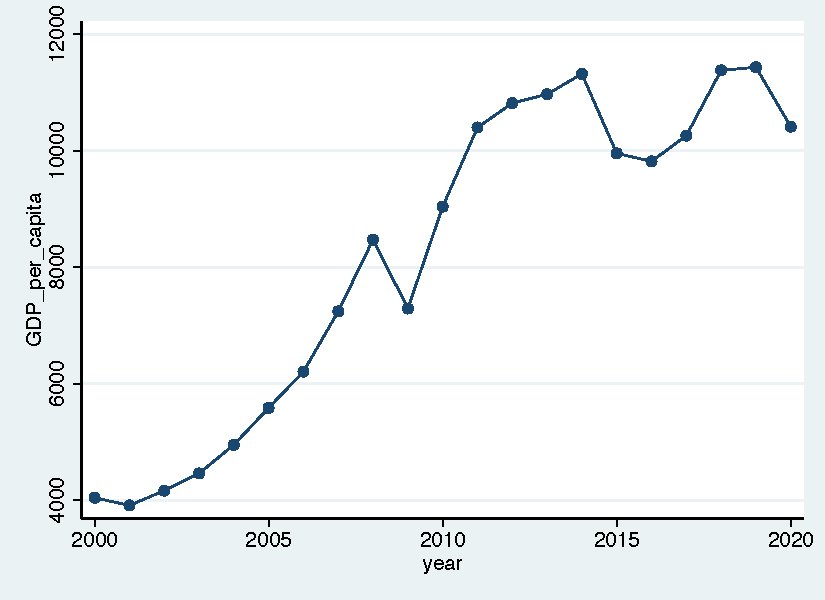
\includegraphics[scale=0.45]{Fig/GDP_per_capita.pdf}\\ % Insert a figure
		\hspace{-9em}\scriptsize{Sources: Worldbank.}\\ % Adjust position and insert sources
		\vspace{-0.5em} % Reduce vertical whitespace
		\caption{GDP per capita in Malaysia (current US\$)} % Figure name
		\label{GDP_per_capita} % Figure label
	\end{figure}
	
\end{frame}

%----------------------------------------------------------------------------------------
%	Table
%----------------------------------------------------------------------------------------

\subsection{Table}
\linespread{1} 
\begin{frame}{\textbf{Insert a Table}}
\linespread{1.5} 

	\begin{table}[htbp]
		\centering 
		\caption{Statistical Differences in Student Loans Between Public and Private Universities in Taiwan (Academic Year 108)} % Table name
		\extrarowheight=2pt % Extra row height
		\label{loan} % Table label
		\scalebox{0.8}{ % Adjust the scale of table
		\begin{tabular}{p{7cm} p{4cm}<{\centering} p{4cm}<{\raggedleft}} % Control column width and text alignment
			\toprule
			\midrule
 			& Public universities & Private universities\\
			\midrule
			Loan amount & 3,121,271,506 & 16,098,465,719 \\
			Number of students with loans & 55,715 & 187,076 \\
			Total number of students & 439,073 & 774,099 \\
			Loan amount per capita & 56,022 & 86,053 \\
			The share of total student & 12.69\% & 24.17\% \\
			\midrule
			\bottomrule
		\end{tabular}
		}
		\par\smallskip
		\hspace{0.5em}\parbox{0.9\textwidth}{\scriptsize % Control the position, font size and box width of source(s) and note(s)
		Source: \href{https://helpdreams.moe.edu.tw/hd/upload/20201211_1.pdf}{Department of Help Dreams}。\par
		Note: \parbox[t]{0.7\textwidth}{\scriptsize % remember to be slightly smaller than the \textwidth of the previous two lines
		You can write a note for the table.
		}
		}
	\end{table}
	
\end{frame}

\linespread{1} 
\begin{frame}{\textbf{Insert a Table (Con't)}}
\linespread{1.5} 

	\begin{table}[htbp]
		\centering 
		\caption{The Best 5 Jobs} 
		\extrarowheight=2pt 
		\label{CareerCast}
		\scalebox{0.7}{ 
		% @{} indicates that the text at the left and right ends of the table is along the edge of the table;
		% lcr can align the text to the left, center, and right respectively, and the width is automatically detected.
		\begin{tabular}{@{}crrrr@{}} 
			\toprule
			\midrule
			 排名 & 2021 &  2019 & 2018 & 2017\\
			\midrule
			1 & {Data Analyst} & \textbf{Data Analyst}  &  Genetic Counselors & \textbf{Statistician} \\
			2 & Genetic Counselors & \textbf{Statistician} & \textbf{Mathematician}  & Medical Services Manager \\
			3 & \textbf{Statistician} & University Professor  & University Professor & \textbf{Operations Research Analyst}\\
			4 &Medical Services Manager & Occupational Therapy  & Occupational Therapy & \textbf{Information Security Analyst} \\
			5 & \textbf{Mathematician} & Genetic Counselors & \textbf{Statistician} & \textbf{Data Analyst} \\
			\midrule
			\bottomrule
		\end{tabular}
		}
		\par\smallskip
		\hspace{0.5em}\parbox{0.93\textwidth}{\scriptsize
		Source: CareerCast, from: \url{https://www.careercast.com}。\par
		Notes: \parbox[t]{0.9\textwidth}{\scriptsize
		1. In 2020, CareerCast did not announce the best jobs of the year.\\
		 2. STEM-related occupations in bold.
		}
		}
	\end{table}

\end{frame}

%----------------------------------------------------------------------------------------
%	Two columns (You can also change it to be three or four...)
%----------------------------------------------------------------------------------------

\section{Two columns}

%----------------------------------------------------------------------------------------

\linespread{1}
\begin{frame}{\textbf{Two columns (or Multiple columns)}}
\linespread{1.5}

	\begin{columns}[c] % Multiple columns
		\column{0.8\textwidth} % Set the column width
			\begin{enumerate}[]
				\item When we refer to previous figures, tables or equations in the text, we should cite them like this:
				\begin{enumerate}[]
					\item ``figure $\backslash$ref\{label\}'', 
						then it will appear figure \ref{GDP_per_capita} and figure \ref{LaTeX}。
					\item ``table $\backslash$ref\{label\}'',
						then it will appear table \ref{loan} and table \ref{CareerCast}。
					\item ``equation ($\backslash$ref\{label\})'',
						then it will appear equation (\ref{reg}) and equation (\ref{var})。
				\end{enumerate}
				\item The advantage of citation is that when the slides are changed, there is no need to manually adjust the numbering all the time.
			\end{enumerate}

		\column{0.2\textwidth} % Set the column width
			\begin{figure}
				
\includegraphics[scale=0.03]{Fig/LaTeX.png}\\
				\scriptsize{Source:
				\href{https://en.wikipedia.org/wiki/LaTeX}{Wiki}。}\\
				\caption{\LaTeX}
				\label{LaTeX} 
			\end{figure}
	\end{columns}
\end{frame}


%----------------------------------------------------------------------------------------
%	Others
%----------------------------------------------------------------------------------------

\begin{frame}

	This is a no title page.\\
	
	\bigskip
		
	Hyperlink buttom: \hyperlink{Link Text}{\beamergotobutton{Link}}
	
\end{frame}

%----------------------------------------------------------------------------------------
%	References
%----------------------------------------------------------------------------------------

\section{References}

%----------------------------------------------------------------------------------------

\linespread{1}  
\begin{frame}{\textbf{Citations}}
\linespread{1.5} 

	Commands for citations:
	
	\begin{enumerate}[1]
		\item textual citations: \textbackslash citet\{label\}。
		\item parenthetical citations: \textbackslash citep\{label\}。
	\end{enumerate}
	
	\bigskip
	
	For instance:
	
	\begin{enumerate}[1]
		\item \citet{Non-CES} and \citet{Melitz (2003)}
		\item \citep{Non-CES} and \citep{Melitz (2003)}
	\end{enumerate}
	
\end{frame}

%----------------------------------------------------------------------------------------

\linespread{1}
\begin{frame}{\textbf{References}}
\linespread{1.5} 

\footnotesize

\begin{thebibliography}{99} 

	\bibitem[K. Matsuyama (2022)]{Non-CES} % citation name{label}
		K. Matsuyama (2022). % Author(s) (year)
		\newblock Non-CES Aggregators: A Guided Tour, % Article name
		\newblock \emph{Annual Review of Economics}, 15, forthcoming. % Periodicals, volume and pages

	\bibitem[Marc J. Melitz (2003)]{Melitz (2003)}
		Marc J. Melitz (2003).
		\newblock The Impact of Trade on Intra-Industry Reallocations and Aggregate Industry Productivity,
		\newblock \emph{Ecometrica},71(6), 1695--1725.
		
\end{thebibliography}

\end{frame}

%----------------------------------------------------------------------------------------
%	Closing Slide
%----------------------------------------------------------------------------------------

\section*{Closing Slide}

%----------------------------------------------------------------------------------------

\begin{frame}[plain] % Hides the headline and footline
	\begin{center}
		{\Huge The End}
		
		\bigskip\bigskip 
		
		{\LARGE Questions? Comments?}
	\end{center}
\end{frame}

%----------------------------------------------------------------------------------------

\end{document} 
